\documentclass[a4paper,12pt]{article}
\usepackage[left=1.25in,right=1.25in,top=1in,bottom=1in]{geometry} % word form
\usepackage[usenames,svgnames,hyperref]{xcolor}
\usepackage{amsmath,array,amsbsy,bm,dashbox,fancybox,graphicx,paralist,slashed,longtable,tabularx,booktabs,floatrow,subfig,tensor}
\usepackage{subfiles}
\usepackage{hyperref}
\hypersetup{colorlinks,linkcolor=blue,citecolor=red}
\linespread{1.25}
%\renewcommand{\rmdefault}{ptm}
\usepackage[T1]{fontenc}
\usepackage{newtxtext, newtxmath}






\begin{document}
\section{SU(3) limit in the trajectory $m_s=m_{s,\mathrm{phy}}$}
In this trajectory, the pion mass in the SU(3) limit is $m_\pi=758$ MeV. The trajectory of the hadron masses is given in Fig.
	\begin{figure}[!htpb]
		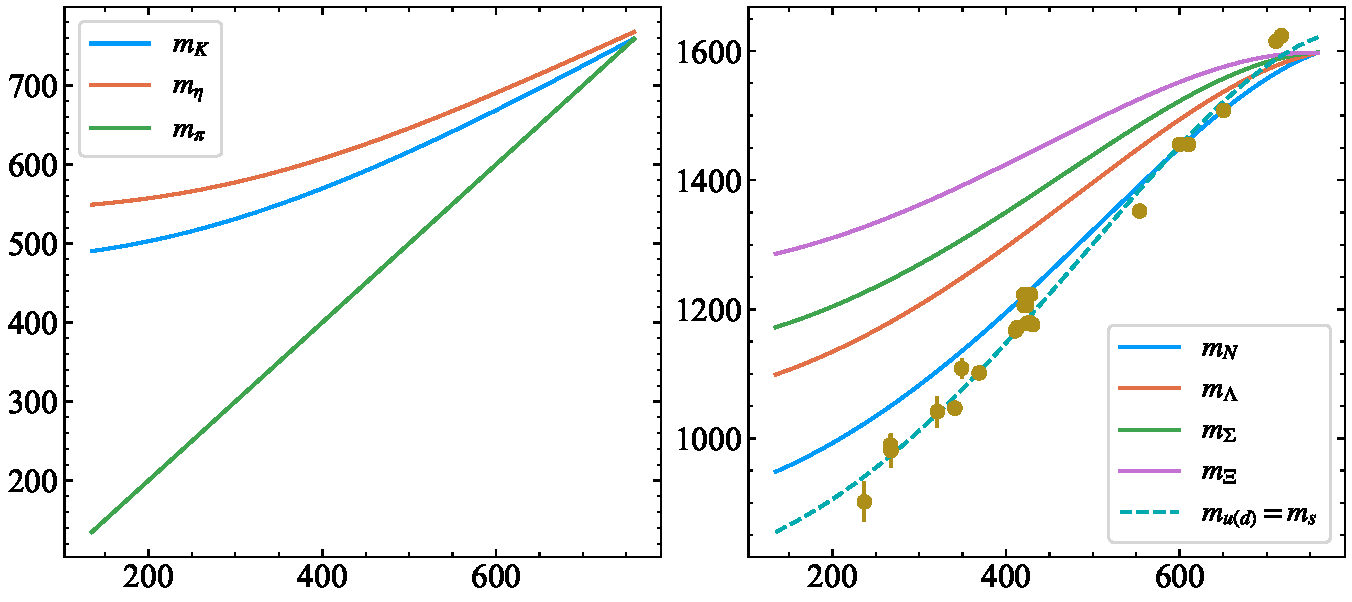
\includegraphics[width=\textwidth]{figure/mh_msphy.pdf}
	\end{figure}
	
	
The trajectories of the two poles of the $\Lambda(1405)$ is given in Fig.

\begin{figure}[!hptb]
	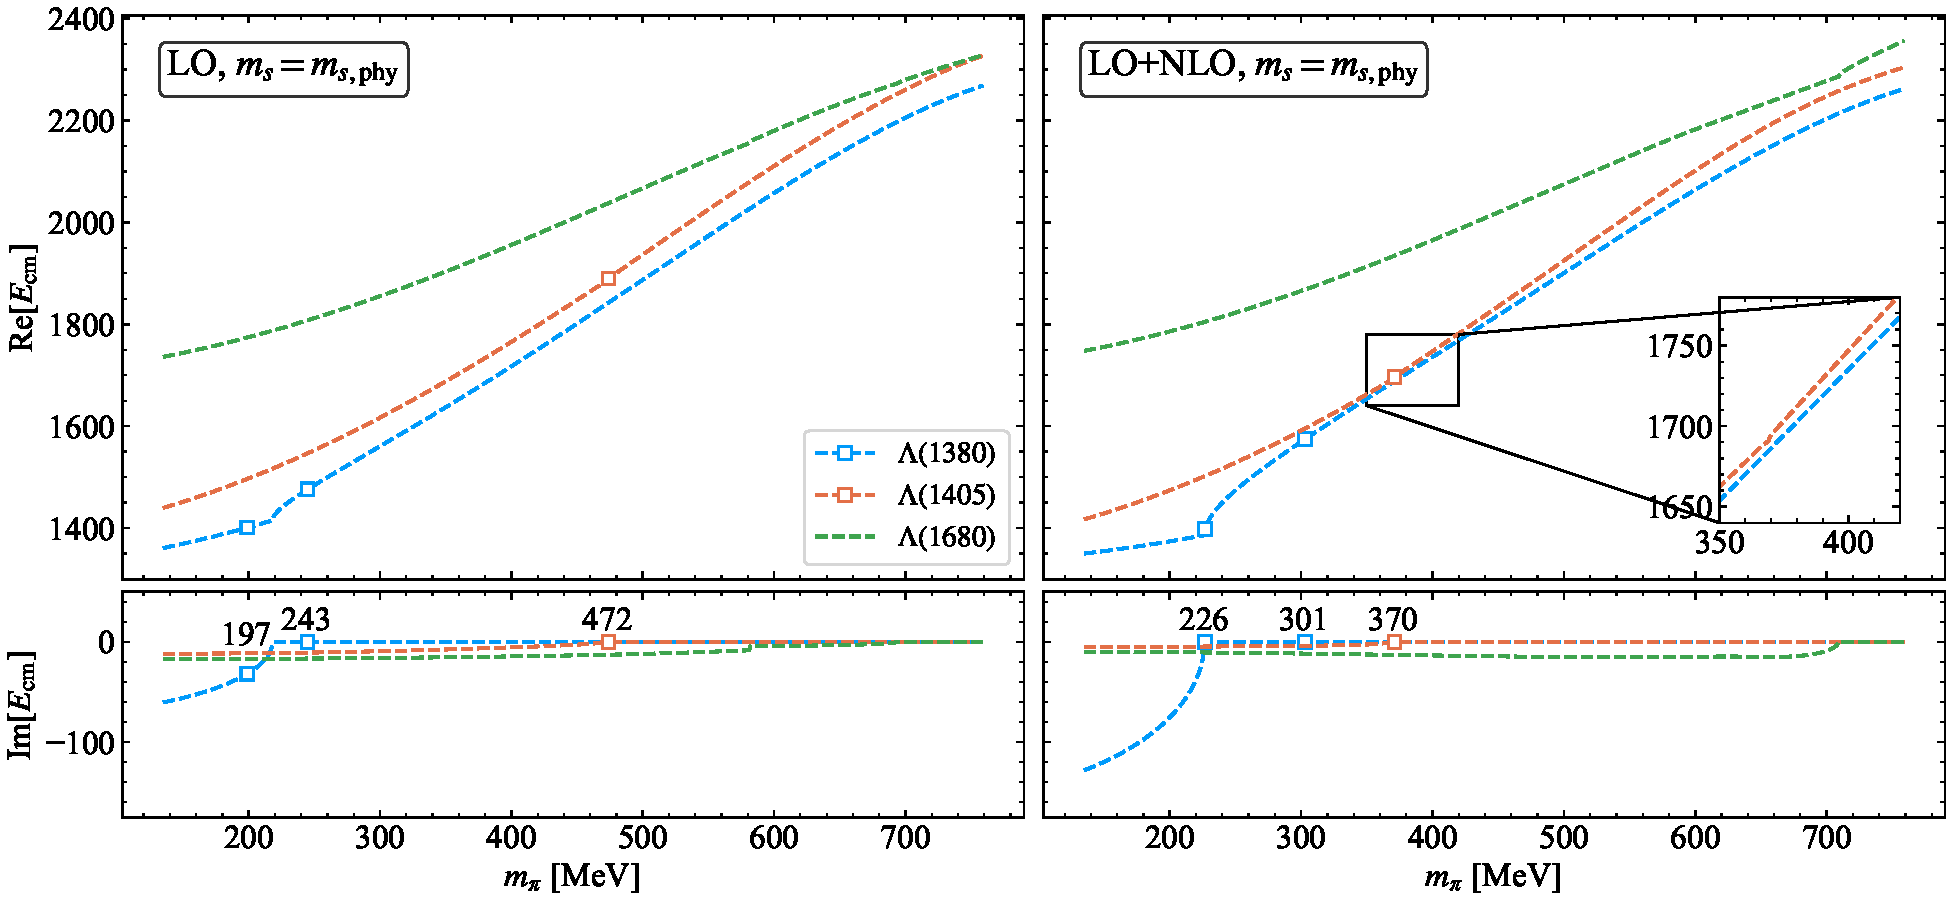
\includegraphics[width=\textwidth]{figure/trajectory_msphy.pdf}
\end{figure}

In the SU(3) limit, the pole positions is given in Table

\begin{table}[!htpb]
\caption{The poles found in the SU(3) limit. Units in MeV. Up to NLO, the third pole is in the unphysical sheet, while other poles are in the physical sheet.}
\begin{centering}

\begin{tabular}{|c|c|c|c|c|}
\hline 
\multicolumn{2}{|c|}{LO} & \multicolumn{3}{c|}{LO+NLO}\tabularnewline
\hline 
\hline 
2268 & 2328 & 2262 & 2304 & 2367(RS$----$)\tabularnewline
\hline 
\end{tabular}
\par\end{centering}
\end{table}






\end{document}